\chapter[Maass Forms and Brownian Motion]{Maass Forms, the Selberg Trace Formula\\ and Brownian Motion on the Modular Surface}\label{ch:maass}

The holomorphic modular forms of Chapter~\ref{ch:02} are half of the automorphic spectrum of $\SL_2(\Z)$. The other half consists of the Maass forms, the eigenfunctions of the hyperbolic Laplacian on the modular surface $X=\SL_2(\Z)\backslash\mathbb H$, and the book has so far mentioned them only in passing. They matter to its programme for two reasons. The first is that the Galois representations on the Maass side are the even ones, which the gamma factor of the Galois heat trace of Chapter~\ref{ch:recip} tells apart from the odd ones (Section~\ref{sec:msquarter}): an even two dimensional Artin representation corresponds, when it corresponds to anything, to a Maass form of eigenvalue exactly $\frac14$, and the even icosahedral case is the one two dimensional case of reciprocity that is open. The second is that the Selberg trace formula, the fundamental identity of the Maass side, is a heat trace identity of precisely the shape of the Galois heat trace of Chapter~\ref{ch:recip}, with closed geodesics in the place of primes, and its probabilistic content is Brownian motion on $X$: the sum of $e^{-t\lambda_j}$ over the Laplace spectrum is the return density of Brownian motion integrated over the surface, decomposed by the homotopy class of the loop the path has made.

This chapter sets out the spectral theory of $X$ in the language of the book. The modular surface is a probability space with the normalised hyperbolic area, Brownian motion on it is ergodic with that law, and the heat kernel decomposes over Maass forms and Eisenstein series. The Selberg trace formula is stated for compact quotients, where it is clean, and read through Brownian loops. Two theorems transcribe the book's dictionary to this setting: Selberg's eigenvalue conjecture is the complete monotonicity of the heat trace, exactly as GRH is the complete monotonicity of the Galois heat trace, and is a theorem for $\SL_2(\Z)$ and within $(\frac7{64})^2$ of a theorem in general; and the closed geodesics, ordered by length, form a Beurling system of primes to which the Poisson Dirichlet theory of Chapter~\ref{ch:pd} and the sine squared lemma of Chapter~\ref{ch:10d} apply without change, so that the geodesic Euler product $Z(s+1)/Z(s)$ is represented unconditionally through a GGC at every basepoint to the right of $1$. The chapter also records an obstruction: Weyl's law places the Laplace spectrum just outside the Thorin class at the centre, because $\sum_j r_j^{-2}$ diverges, whereas $\sum_\gamma\gamma^{-2}$ over the zeros of an $L$ function converges. The last section states and checks the Eichler Selberg trace formula, the holomorphic analogue that Chapter~\ref{ch:07} uses, and reads it as the moment identity behind Serre's vertical Sato Tate law.

\section{The modular surface as a probability space}\label{sec:mssurface}

Let $\mathbb H=\{z=x+iy:\ y>0\}$ with the hyperbolic metric $ds^2=(dx^2+dy^2)/y^2$, area element $d\mu=dx\,dy/y^2$, and Laplacian
\[
\Delta=-y^2\Bigl(\frac{\partial^2}{\partial x^2}+\frac{\partial^2}{\partial y^2}\Bigr),
\]
a nonnegative operator in the sign convention of this chapter. The group $\SL_2(\R)$ acts by isometries, and $\Gamma=\SL_2(\Z)$ acts with the fundamental domain $F=\{|x|\le\frac12,\ |z|\ge1\}$ of area $\pi/3$. The modular surface $X=\Gamma\backslash\mathbb H$ carries the probability measure $\frac3\pi d\mu$; this is the probability space of the chapter. Under it the height $y$ has a heavy tail, $\Prob(y>Y)=3/(\pi Y)$ for $Y\ge1$, so that $y$ has no mean: the cusp carries a vanishing fraction of the area at great height, but not a summable one.

A \emph{Maass form}\index{Maass form} is a $\Gamma$ invariant eigenfunction of $\Delta$ of moderate growth; a Maass cusp form has vanishing constant term in its Fourier expansion, hence is square integrable and decays exponentially in the cusp. The spectral theorem for $L^2(X)$ (Selberg) says that $L^2(X)$ is the orthogonal sum of the constants, of the closed span of the Maass cusp forms $u_j$ with eigenvalues $\lambda_j=\frac14+r_j^2$, $0<\lambda_1\le\lambda_2\le\cdots$, and of the continuous spectrum $[\frac14,\infty)$ spanned by the Eisenstein series $E(z,\frac12+ir)$, $r\in\R$. For $\SL_2(\Z)$ every cuspidal eigenvalue exceeds $\frac14$, so every $r_j$ is real, and the first few are
\begin{gather*}
r_j=9.533695,\ 12.173008,\ 13.779751,\ 14.358510,\\
16.138073,\ 16.644259,\ 17.738563,\ 18.180918,
\end{gather*}
with $\lambda_1=91.141$; the first form is odd and the first even form, invariant under $x\mapsto-x$, is the third. The eigenvalues are known to many digits \cite{hejhal1992,lmfdb} and have been certified rigorously \cite{bookerstrombergssonvenkatesh2006}; the first hundred, $61$ odd and $39$ even, are shown in Figure~\ref{fig:msspectrum}. Weyl's law for $X$, due to Selberg, is
\begin{equation}\label{eq:msweyl}
N(T)=\#\{j:\ r_j\le T\}=\frac{T^2}{12}-\frac{2T}{\pi}\log T+O(T),
\end{equation}
the leading term being $\frac{\operatorname{area}(X)}{4\pi}T^2$, so that the cusp forms are as numerous as the eigenfunctions of a compact surface of the same area: the continuous spectrum takes up none of Weyl's count. This is special to congruence groups and is the analytic reason the spectral theory of $X$ is arithmetic. The first hundred eigenvalues reach $r=46$, where $T^2/12=176$ and the logarithmic term has removed $112$; the remaining linear term is about $0.78T$ at this height (Figure~\ref{fig:msspectrum}).

\begin{figure}[t]
\centering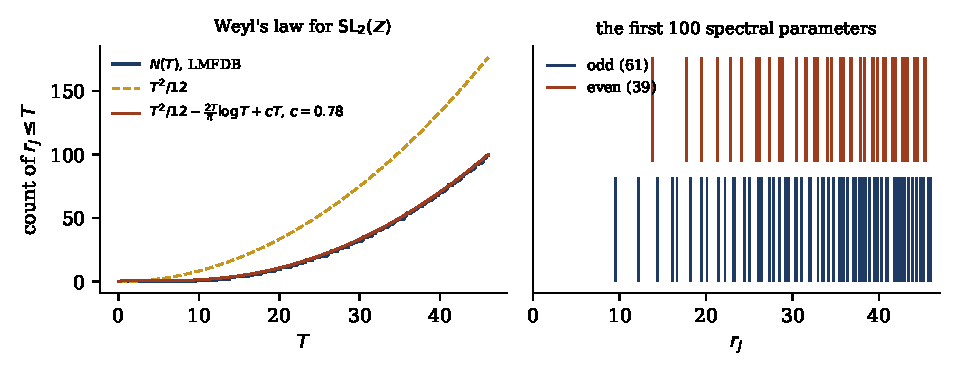
\includegraphics[width=\textwidth]{figs/maass_spectrum.pdf}
\caption{The cuspidal spectrum of $\SL_2(\Z)$. Left: the counting function $N(T)$ of the first hundred spectral parameters against $T^2/12$ and against Weyl's law with its logarithmic term and a fitted linear term. Right: the spectral parameters themselves, odd forms below and even forms above.}\label{fig:msspectrum}
\end{figure}

The Hecke operators $T_n$ commute with $\Delta$ and with each other, so the cusp forms can be taken to be Hecke eigenforms, $T_nu_j=\lambda_j(n)u_j$, with Fourier expansions $u_j(z)=\sum_{n\ne0}\rho_j(n)\sqrt y\,K_{ir_j}(2\pi|n|y)e^{2\pi inx}$ and $\rho_j(n)=\rho_j(1)\lambda_j(n)$ for $n\ge1$. The $L$ function $L(s,u_j)=\sum_{n\ge1}\lambda_j(n)n^{-s}$ has the Euler product $\prod_p(1-\lambda_j(p)p^{-s}+p^{-2s})^{-1}$, Satake parameters $\alpha_p,\alpha_p^{-1}$ with $\alpha_p+\alpha_p^{-1}=\lambda_j(p)$, and the completed function
\[
\Lambda(s,u_j)=\Gamma_\R(s+\epsilon_j+ir_j)\Gamma_\R(s+\epsilon_j-ir_j)L(s,u_j)=(-1)^{\epsilon_j}\Lambda(1-s,u_j),
\]
$\epsilon_j\in\{0,1\}$ the parity, is entire. In the normalisation of Section~\ref{sec:10bcompletion} the archimedean parameters are $\mu=\epsilon_j\pm ir_j$, and $u_j$ generates a cuspidal automorphic representation of $\GL_2(\A_\Q)$, so Theorem~\ref{thm:10bmain} applies: GRH for $L(s,u_j)$ is equivalent to $\Xi_{u_j}(0)/\Xi_{u_j}(\sqrt\lambda)$ being a GGC transform, and Theorem~\ref{thm:10dshift} gives the Thorin representation at every basepoint $\alpha\ge1$ unconditionally.

Two conjectures govern the Maass side and both are statements about the Thorin framework. The \emph{Ramanujan conjecture}\index{Ramanujan conjecture!for Maass forms} for Maass forms is $|\lambda_j(p)|\le2$, that is $|\alpha_p|=1$; for holomorphic forms this is Deligne's theorem, for Maass forms the best known bound is Kim and Sarnak's $|\alpha_p|\le p^{7/64}$ \cite{kimsarnak2003}. \emph{Selberg's eigenvalue conjecture}\index{Selberg's eigenvalue conjecture} is that $\lambda_1\ge\frac14$ for every congruence subgroup, that is that no $r_j$ is imaginary; it is the archimedean Ramanujan conjecture, and Kim and Sarnak's bound gives $\lambda_1\ge\frac14-(\frac7{64})^2=\frac{975}{4096}$. For $\SL_2(\Z)$ itself $\lambda_1=91.14$ and the conjecture is trivially true; the content is in the groups $\Gamma_0(N)$ and $\Gamma(N)$ as $N$ grows.

\begin{corollary}[Ramanujan at $p$ is local Thorin positivity]\label{cor:msramanujan}
Let $u$ be a Hecke Maass eigenform and $p$ a prime. The function
\[
\lambda\mapsto\frac{2-\lambda(p)}{p^{\sqrt\lambda}+p^{-\sqrt\lambda}-\lambda(p)}=(2-\lambda(p))\,p^{-\sqrt\lambda}L_p(\sqrt\lambda,u),
\]
where $L_p(s,u)=(1-\lambda(p)p^{-s}+p^{-2s})^{-1}$ is the Euler factor,
is the Laplace transform of a probability law on $[0,\infty)$ if and only if $-2\le\lambda(p)<2$, in which case the law is the GGC with Thorin comb $\sum_{k\in\Z}\delta_{t_k}$, $t_k=((\theta_p+2\pi k)/\log p)^2$, $\lambda(p)=2\cos\theta_p$. In particular the Ramanujan conjecture at $p$ (with $\lambda(p)\ne2$) holds if and only if the local factor of $u$ at $p$ is a GGC transform in the variable $\sqrt\lambda$.
\end{corollary}

\begin{proof}
$L_p(s,u)^{-1}=1-\lambda(p)p^{-s}+p^{-2s}=p^{-s}(p^s+p^{-s}-\lambda(p))$, so the displayed function is $f_x$ of Theorem~\ref{thm:10clocal} with $x=\lambda(p)$ and $L=\log p$.
\end{proof}

For holomorphic forms the corollary is a theorem at every $p$, by Deligne; for Maass forms it is known only that $\lambda(p)\in[-p^{7/64}-p^{-7/64},p^{7/64}+p^{-7/64}]$, and whether every local factor of every Maass form is a GGC transform is the Ramanujan conjecture itself. Numerically every Hecke eigenvalue ever computed for a Maass form satisfies the bound.

\section{Brownian motion and the heat kernel}\label{sec:msbm}

Brownian motion on $\mathbb H$ is the diffusion with generator $-\Delta=y^2(\partial_x^2+\partial_y^2)$, so that its transition density solves $\partial_tu=-\Delta u$; it is the standard Brownian motion of the metric run at twice the usual speed, which is the convention that makes the heat kernel $e^{-t\Delta}$. In coordinates it solves
\[
dx_t=\sqrt2\,y_t\,dB^1_t,\qquad d\log y_t=\sqrt2\,dB^2_t-dt,
\]
so that $\log y$ is a Brownian motion with drift $-1$ and the process drifts towards the real axis in the half plane, while on $X$ the identification by $\Gamma$ returns it from the cusp. The heat kernel on $\mathbb H$ depends only on the distance $\rho=d(z,w)$ and is (McKean \cite{mckean1972})
\begin{equation}\label{eq:msmckean}
p_t(\rho)=\frac{\sqrt2\,e^{-t/4}}{(4\pi t)^{3/2}}\int_\rho^\infty\frac{s\,e^{-s^2/4t}}{\sqrt{\cosh s-\cosh\rho}}\,ds ,
\end{equation}
with $p_t(0)\sim(4\pi t)^{-1}$ as $t\to0$, the Euclidean value in two dimensions, $p_t(0)\sim\sqrt\pi e^{-t/4}/(8t^{3/2})$ as $t\to\infty$ (Figure~\ref{fig:msheat}), and $p_t(\rho)\asymp t^{-3/2}e^{-t/4-\rho^2/4t-\rho/2}$ up to polynomial factors in $\rho$ and $t$ at large $t$ and $\rho$, the factor $e^{-t/4}$ being the bottom of the spectrum of $\Delta$ on $\mathbb H$. The heat kernel on $X$ is the sum over the group,
\begin{equation}\label{eq:msimages}
K_t(z,w)=\sum_{\gamma\in\bar\Gamma}p_t(d(z,\gamma w)),\qquad\bar\Gamma=\Gamma/\{\pm1\},
\end{equation}
and has the spectral expansion
\begin{equation}\label{eq:msspectral}
\begin{split}
K_t(z,w)={}&\frac3\pi+\sum_{j\ge1}e^{-t\lambda_j}u_j(z)\overline{u_j(w)}\\
&+\frac1{4\pi}\int_{-\infty}^\infty e^{-t(\frac14+r^2)}E(z,\tfrac12+ir)\overline{E(w,\tfrac12+ir)}\,dr .
\end{split}
\end{equation}

\begin{figure}[t]
\centering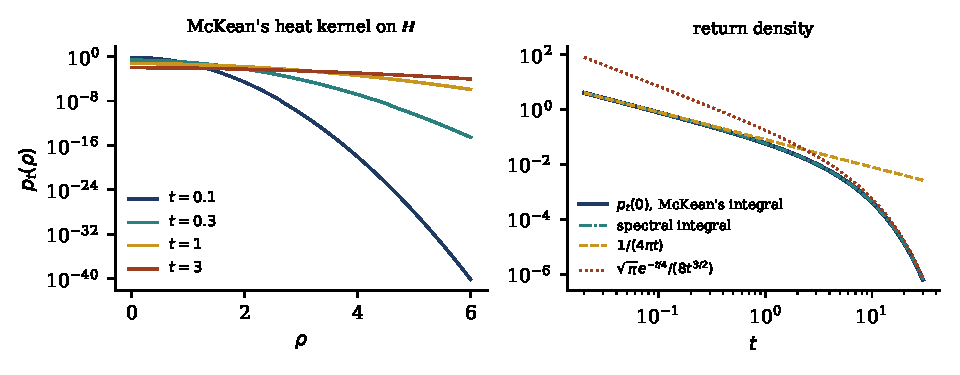
\includegraphics[width=\textwidth]{figs/maass_heat.pdf}
\caption{McKean's heat kernel on $\mathbb H$. Left: $p_t(\rho)$ as a function of the distance $\rho$ for four values of $t$. Right: the return density $p_t(0)$ from \eqref{eq:msmckean} and from the spectral integral $\frac1{4\pi}\int_{\R}e^{-t(1/4+r^2)}r\tanh(\pi r)\,dr$, which agree to $10^{-4}$, between the small time asymptote $1/(4\pi t)$ and the large time asymptote $\sqrt\pi e^{-t/4}/(8t^{3/2})$, whose exponential rate $\frac14$ is the bottom of the spectrum.}\label{fig:msheat}
\end{figure}

\begin{proposition}[Brownian motion on $X$]\label{prop:msergodic}
Brownian motion on $X$ is a positive recurrent diffusion with invariant probability $\frac3\pi d\mu$, and for every $f\in L^1(X,\mu)$, $\frac1T\int_0^Tf(B_s)\,ds\to\frac3\pi\int_Xf\,d\mu$ almost surely. The law of $B_t$ started anywhere converges to $\frac3\pi d\mu$ in total variation, at the rate $e^{-t\lambda_1}$ in $L^2$ with $\lambda_1=91.14$ for the cuspidal part, and at the rate of the continuous spectrum, $e^{-t/4}$ up to a power of $t$, for the Eisenstein part, which is the time it takes the process to come back from the cusp.
\end{proposition}

\begin{proof}
Positive recurrence follows from finiteness of the area and the spectral gap of $\Delta$ on cusp forms together with the explicit form of the continuous spectrum: $\int_XK_t(z,w)f(w)\,d\mu(w)-\frac3\pi\int f\,d\mu$ is bounded in $L^2$ by $e^{-t\lambda_1}\|f\|_2$ for the cuspidal projection and by $e^{-t/4}$ times a power of $t$ for the Eisenstein projection, from \eqref{eq:msspectral}. The ergodic theorem is Birkhoff's for a positive recurrent diffusion.
\end{proof}

The Euler scheme for the stochastic differential equation, with step $10^{-3}$, each step followed by reduction to $F$, gives for $64$ paths run to time $2\cdot10^4$ the time fractions $\Prob(y>1)=0.9551$, $\Prob(y>2)=0.4784$, $\Prob(y>4)=0.2397$, $\Prob(y>8)=0.1201$ against $3/(\pi Y)=0.9549$, $0.4775$, $0.2387$, $0.1194$, and the empirical density of $y$ on $[1,32]$ agrees with $3/(\pi y^2)$ to within $1.1$ percent in every one of twenty logarithmic bins (Figure~\ref{fig:msbm}). The time average of $y^{-1}\mathsf 1_{y\ge1}$ is $0.4769$ against $3/2\pi=0.4775$.

\begin{figure}[t]
\centering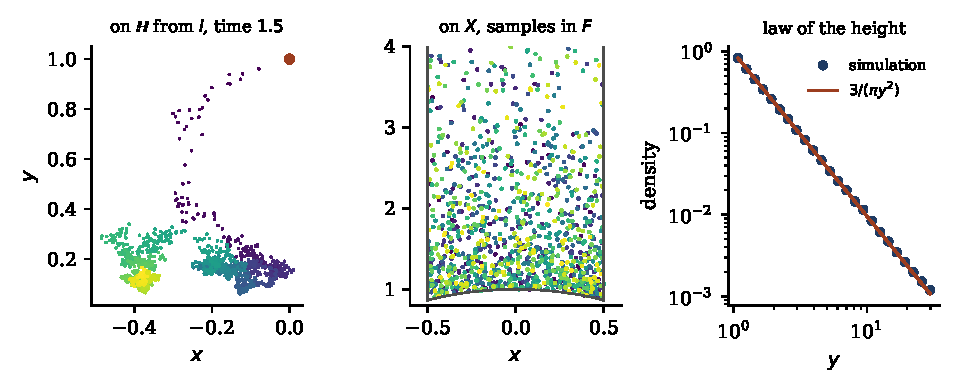
\includegraphics[width=\textwidth]{figs/maass_bm.pdf}
\caption{Brownian motion on the modular surface. Left: a path of the hyperbolic Brownian motion in $\mathbb H$ started at $i$, run to time $1.5$; the drift of $\log y$ carries it towards the real axis. Middle: the process on $X$, every fiftieth sample point in the fundamental domain, coloured by time, filling the domain according to the hyperbolic area. Right: the empirical law of the height $y$ along the path against the density $3/(\pi y^2)$ of the normalised hyperbolic area for $y\ge1$.}\label{fig:msbm}
\end{figure}

\section{The Selberg trace formula as a heat trace}\label{sec:msstf}

For a compact quotient the trace of the heat kernel is both a spectral and a geometric sum, and that is the trace formula. Let $\Gamma$ be a discrete subgroup of $\SL_2(\R)$ acting without fixed points with compact quotient $X_\Gamma$ of genus $g\ge2$, area $4\pi(g-1)$, and Laplace eigenvalues $0=\lambda_0<\lambda_1\le\cdots$, $\lambda_j=\frac14+r_j^2$. Every nontrivial conjugacy class in $\Gamma$ is hyperbolic and is a power $P^k$ of a primitive class $P$, which corresponds to a primitive closed geodesic of length $\ell(P)$; put $N(P)=e^{\ell(P)}$, the norm.

\begin{theorem}[Selberg \cite{selberg1956}; heat kernel form]\label{thm:msstf}
For every $t>0$,
\begin{equation}\label{eq:msstf}
\begin{split}
\sum_{j\ge0}e^{-t\lambda_j}={}&\frac{\operatorname{area}(X_\Gamma)}{4\pi}\int_{-\infty}^\infty e^{-t(\frac14+r^2)}\,r\tanh(\pi r)\,dr\\
&+\sum_P\sum_{k\ge1}\frac{\ell(P)}{2\sinh(k\ell(P)/2)}\,\frac{e^{-t/4}e^{-(k\ell(P))^2/4t}}{\sqrt{4\pi t}} .
\end{split}
\end{equation}
\end{theorem}

This is the general trace formula
\[
\sum_jh(r_j)=\frac{\operatorname{area}}{4\pi}\int h(r)\,r\tanh(\pi r)\,dr+\sum_{P,k}\frac{\ell(P)}{2\sinh(k\ell(P)/2)}\,g(k\ell(P)),
\]
with $g(u)=\frac1{2\pi}\int h(r)e^{-iru}\,dr$, applied to $h(r)=e^{-t(1/4+r^2)}$, for which $g(u)=e^{-t/4}e^{-u^2/4t}/\sqrt{4\pi t}$. For the modular surface the same identity holds with elliptic terms for the two elliptic points, parabolic terms for the cusp, and the spectral side carrying the continuous spectrum through the scattering determinant; the statement is in Hejhal \cite{hejhal1983} and Iwaniec \cite{iwaniec2002}, and the structure is the same.

The probabilistic reading is McKean's \cite{mckean1972}, and the book's dictionary makes it exact. By \eqref{eq:msimages} and \eqref{eq:msspectral},
\[
\sum_je^{-t\lambda_j}=\int_{X_\Gamma}K_t(z,z)\,d\mu(z)=\int_{X_\Gamma}\sum_\gamma p_t(d(z,\gamma z))\,d\mu(z).
\] The term $\gamma=1$ is $\operatorname{area}\cdot p_t(0)$, the return density of free Brownian motion on $\mathbb H$ integrated over the surface, and \eqref{eq:msmckean} integrated against $\tanh$ is the statement $p_t(0)=\frac1{4\pi}\int e^{-t(1/4+r^2)}r\tanh(\pi r)\,dr$, the spectral density of $\Delta$ on $\mathbb H$. The terms $\gamma\sim P^k$ collect, for each $z$, the density at $z$ of Brownian paths from $z$ that return to $z$ in the free homotopy class of the closed geodesic $P^k$: a path from $z$ to $\gamma z$ in $\mathbb H$ is a loop on $X_\Gamma$ in the class of $\gamma$. Integrating over a fundamental domain of the centraliser of $P$ gives the factor $\ell(P)/(2\sinh(k\ell(P)/2))$, and $g(k\ell(P))$ is the one dimensional Gaussian density at distance $k\ell(P)$ with the spectral shift $e^{-t/4}$. So \eqref{eq:msstf} says: the total return probability of Brownian motion on $X_\Gamma$ equals the free return probability plus the sum over closed geodesics of the probability of returning around that geodesic. Compare the Galois heat trace of Definition~\ref{def:recipheat},
\[
\begin{split}
\mathcal W_\rho(x)={}&\frac1{4\pi}\int e^{-xr^2}\Bigl(\log N_\rho+2\operatorname{Re}\frac{\gamma'}\gamma(\tfrac12+ir,\rho)\Bigr)dr\\
&-\frac1{2\sqrt{\pi x}}\sum_{n\ge2}\frac{\Lambda_\rho(n)}{\sqrt n}\,e^{-(\log n)^2/4x},
\end{split}
\]
which equals $\frac12\sum e^{-x\gamma^2}$ over the zeros $\frac12+i\gamma$ (Theorem~\ref{thm:recipcm}). The two formulas have the same three parts: a spectral sum ($e^{-tr_j^2}$ over eigenvalues, $e^{-x\gamma^2}$ over zeros), an archimedean integral ($r\tanh\pi r$, $\gamma'/\gamma$), and a sum over primes ($\log N(P)=\ell(P)$ with the Gaussian $e^{-(k\ell)^2/4t}$, $\Lambda(n)=\log p$ with $e^{-(\log n)^2/4x}$). The one difference is the sign of the prime sum, and it is explained by the Selberg zeta function below: $Z$ is built like $1/\zeta$, so its logarithmic coefficients are $-\ell(P)$ where those of $\zeta$ are $+\log p$.

\begin{theorem}[Selberg's conjecture as complete monotonicity; this book]\label{thm:mscm}
Let $\Gamma$ be a congruence subgroup of $\SL_2(\Z)$ and $\Theta_\Gamma(t)=\sum_{j\ge1}e^{-t\lambda_j}$ the heat trace over the Maass cusp forms, $\lambda_j=\frac14+r_j^2$.
\begin{enumerate}
\item[(i)] $e^{t/4}\Theta_\Gamma(t)=\sum_je^{-tr_j^2}$ is completely monotone on $(0,\infty)$ if and only if $\lambda_j\ge\frac14$ for every $j$, that is if and only if Selberg's eigenvalue conjecture holds for $\Gamma$; in that case its Bernstein measure is $\sum_j\delta_{r_j^2}$.
\item[(ii)] Unconditionally, $e^{t(\frac14-(7/64)^2)}\Theta_\Gamma(t)$ is completely monotone.
\item[(iii)] For $\Gamma=\SL_2(\Z)$, (i) holds, and $\sum_je^{-tr_j^2}\sim\frac1{12t}$ as $t\to0$.
\item[(iv)] The measure $\sum_j\delta_{r_j^2}$ is not a Thorin measure: $\sum_jr_j^{-2}=\infty$.
\end{enumerate}
\end{theorem}

\begin{proof}
(i) By Weyl's law the series converges for $t>0$. If every $r_j^2\ge0$ the function is a Laplace transform of a positive measure, hence completely monotone by Bernstein's theorem, with the stated Bernstein measure by uniqueness. If some $\lambda_j<\frac14$ then $r_j^2<0$ and the corresponding term grows exponentially, so the function is not bounded as $t\to\infty$, while a completely monotone function is decreasing. (ii) is (i) applied with the shift $\frac14-(\frac7{64})^2$, since $\lambda_j\ge\frac{975}{4096}$ by Kim and Sarnak. (iii) The first statement is $\lambda_1=91.14$; the asymptotic is Karamata's Tauberian theorem applied to \eqref{eq:msweyl}, or directly the identity term of the trace formula, $\frac{\operatorname{area}}{4\pi}\int e^{-tr^2}r\tanh(\pi r)\,dr\sim\frac{\operatorname{area}}{4\pi t}=\frac1{12t}$. (iv) By Weyl's law for $\Gamma$, $N(T)\sim\frac{\operatorname{area}}{4\pi}T^2$, of which \eqref{eq:msweyl} is the case $\SL_2(\Z)$, the sum $\sum_jr_j^{-2}=\int_1^\infty T^{-2}\,dN(T)$ diverges like $\frac{\operatorname{area}}{2\pi}\log T$ (like $\frac16\log T$ for $\SL_2(\Z)$), so the second integrability condition of Definition~\ref{def:ch10ggc}, $\int_{(1,\infty)}t^{-1}\tau(dt)<\infty$, fails.
\end{proof}

Theorem~\ref{thm:mscm} is Theorem~\ref{thm:recipcm} with eigenvalues for zeros, and on the Maass side much of the analogue of the Riemann hypothesis comes free: the Laplacian is self adjoint and the Hecke operators commute with it, so every $r_j^2$ is real and the only possible exceptions are finitely many eigenvalues $\lambda_j<\frac14$, which is the whole content of the Maass side being spectral. Selberg's conjecture, that there are none, is open in general; it holds for $\SL_2(\Z)$, which gives part (iii), and part (ii) is what the bound of Kim and Sarnak gives for every congruence subgroup. Part (iv) is the limit of the analogy. The zeros of an $L$ function of degree $n$ have counting function $\frac{nT}{2\pi}\log T$, a one dimensional spectrum, and $\sum\gamma^{-2}$ converges, so Theorem~\ref{thm:10bmain} can place them in a Thorin measure. The eigenvalues of a surface have a two dimensional count, $\sum r_j^{-2}$ diverges logarithmically, and the function $\prod_j(1+\lambda/r_j^2)$ does not converge; the Selberg zeta function is of order two, and no GGC has it for a Laplace transform. The heat trace is the right object, and the Thorin framework enters, as the next section shows, through the Euler product and not through the spectrum.

\section{Closed geodesics as primes}\label{sec:msgeodesics}

The Selberg zeta function\index{Selberg zeta function} of $\Gamma$ is
\[
Z(s)=\prod_P\prod_{k\ge0}\bigl(1-N(P)^{-s-k}\bigr),\qquad\operatorname{Re}s>1,
\]
the product over primitive hyperbolic classes. It continues to an entire function of order two (compact case; meromorphic for $\SL_2(\Z)$), with zeros at $s_j=\frac12\pm ir_j$ for each eigenvalue $\lambda_j=\frac14+r_j^2$, a simple zero at $s=1$ from $\lambda_0=0$, and zeros at the nonpositive integers of multiplicity growing linearly; for $\SL_2(\Z)$ there are in addition zeros at $s=\rho/2$ for the nontrivial zeros $\rho$ of $\zeta$, coming from the scattering determinant $\varphi(s)=\sqrt\pi\,\Gamma(s-\frac12)\zeta(2s-1)/(\Gamma(s)\zeta(2s))$. For a congruence subgroup the zeros $s_j$ lie on $\operatorname{Re}s=\frac12$ if and only if Selberg's eigenvalue conjecture holds, and for $\SL_2(\Z)$ the additional zeros $\rho/2$ lie on $\operatorname{Re}s=\frac14$ if and only if the Riemann hypothesis holds; a compact surface may have eigenvalues below $\frac14$, and then $Z$ has real zeros in $(\frac12,1)$.

The ratio
\begin{equation}\label{eq:msR}
R(s)=\frac{Z(s+1)}{Z(s)}=\prod_P\bigl(1-N(P)^{-s}\bigr)^{-1}=\sum_{\mathfrak n}N(\mathfrak n)^{-s}
\end{equation}
is an Euler product of the shape of $\zeta$, the sum running over the free abelian monoid generated by the primitive geodesics, whose elements we call \emph{geodesic integers}\index{geodesic integer} and whose norms are multiplicative. The prime geodesic theorem,
\[
\pi_\Gamma(x)=\#\{P:\ N(P)\le x\}=\operatorname{li}(x)+O(x^{3/4+\epsilon})
\]
for the modular surface, is due to Huber and Selberg for compact surfaces, where the terms $\operatorname{li}(x^{s_j})$ of the eigenvalues $\lambda_j<\frac14$ are added, and to Sarnak for $\SL_2(\Z)$ \cite{sarnak1982}, where the exponent has since been lowered to $\frac{25}{36}$ \cite{soundararajanyoung2013}; the primitive geodesics of $\SL_2(\Z)$ correspond to the narrow classes of primitive binary quadratic forms of positive nonsquare discriminant $d$, with $N(P)=\epsilon_d^2$ for the smallest unit $\epsilon_d>1$ of norm $+1$ in the order of discriminant $d$, so that $\pi_\Gamma(x)=\sum_{\epsilon_d\le\sqrt x}h^+(d)$ and the theorem is a statement about class numbers of indefinite forms. Enumerating the discriminants to $4\cdot10^6$ with their units and class numbers gives $78441$ primitive geodesics of norm at most $10^6$, against $\operatorname{li}(10^6)=78628$, ratio $0.9976$, and $\sum_{N(P)^k\le x}\ell(P)=0.9991x$ at $x=10^6$ (Figure~\ref{fig:msgeodesics}, left); the shortest geodesic has $N(P)=\varphi^4=6.854$, $\varphi$ the golden ratio, from the discriminant $5$, and the second shortest has norm $13.93$ with multiplicity two, from the discriminant $12$ whose order has no unit of norm $-1$.

\begin{figure}[t]
\centering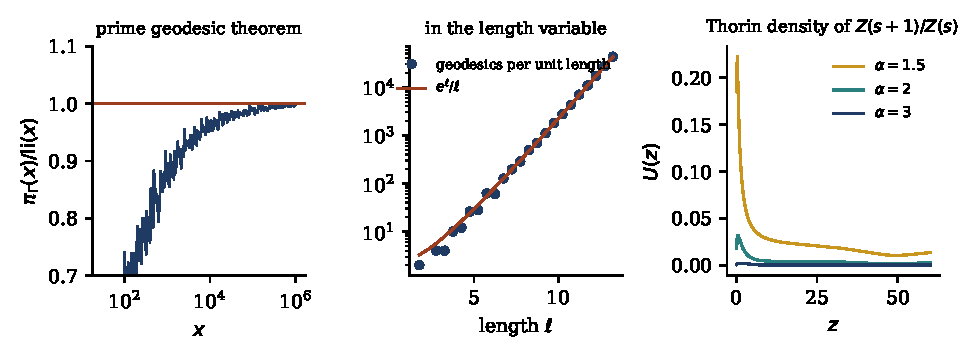
\includegraphics[width=\textwidth]{figs/maass_geodesics.pdf}
\caption{Left: the prime geodesic theorem on the modular surface, $\pi_\Gamma(x)/\operatorname{li}(x)$ for $x\le10^6$ from the class numbers and units of the $2\cdot10^6$ discriminants below $4\cdot10^6$. Middle: the number of primitive geodesics per unit length against $e^\ell/\ell$, the prime geodesic theorem in the length variable. Right: the Thorin density $U(z)$ of the geodesic Euler product $Z(s+1)/Z(s)$ at the basepoints $\alpha=1.5$, $2$ and $3$, from Theorem~\ref{thm:msthorin}; it is positive and integrable, and at $\alpha=2$ its integral against $\log(1+z/t)$ reproduces $\log(R(2)/R(2+\sqrt z))$ to between $10^{-7}$ and $10^{-5}$.}\label{fig:msgeodesics}
\end{figure}

The eigenvalues are visible in the geodesic count. The explicit formula for the modular surface, which is the trace formula with a sharp cutoff for $h$, gives $\psi_\Gamma(x)=\sum_{N(P)^k\le x}\ell(P)=x+\sum_jx^{s_j}/s_j+\cdots$ with $s_j=\frac12\pm ir_j$, so that $(\psi_\Gamma(x)-x)/\sqrt x$ is, up to smaller terms, the almost periodic function $\sum_j2\operatorname{Re}(x^{ir_j}/s_j)$ of $u=\log x$, with frequencies the $r_j$ and amplitudes about $2/r_j$. Figure~\ref{fig:mszeta} shows this function on $50\le x\le10^6$ and its periodogram in $u$: the largest peak below $r=19$ is at $r=9.53$, the first eigenvalue, and the next peaks are at $12.13$, $14.11$ and $16.27$, where the resolution $2\pi/\log(2\cdot10^4)\approx0.6$ of a window of length $\log(2\cdot10^4)$ does not separate the pairs $13.78$, $14.36$ and $16.14$, $16.64$. This is the prime side hearing the spectral side, Weil's explicit formula read backwards, and it is the arithmetic content of Theorem~\ref{thm:msstf}. The right panel of the figure shows the two terms of the heat trace formula as functions of $t$, the identity term $\sim1/(12t)$ at small $t$ and the geodesic sum, which is $O(e^{-\ell_1^2/4t})$ at small $t$ and overtakes the identity term only for $t$ of order one, where the whole trace is dominated by $\lambda_0=0$.

\begin{figure}[t]
\centering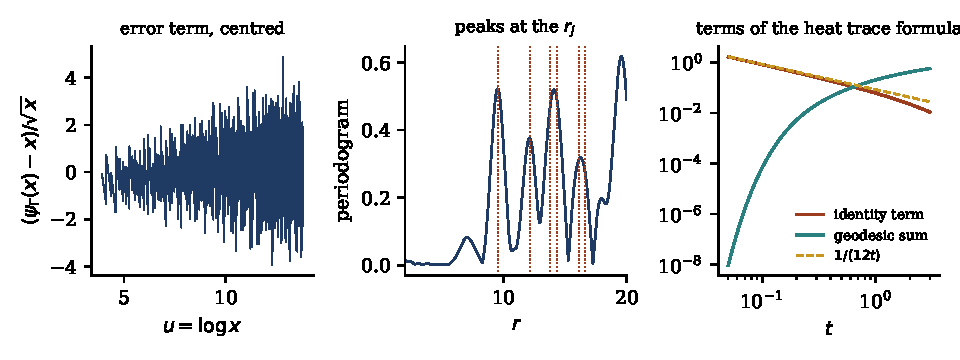
\includegraphics[width=\textwidth]{figs/maass_zeta.pdf}
\caption{The spectrum in the geodesics. Left: the error term $(\psi_\Gamma(x)-x)/\sqrt x$ of the prime geodesic theorem, centred, as a function of $u=\log x$. Middle: its periodogram in $u$, with the first six eigenvalue parameters $r_j$ marked; the peak at $9.53$ is the first Maass form. Right: the identity term and the geodesic sum of the heat trace formula \eqref{eq:msstf} for the modular surface as functions of $t$.}\label{fig:mszeta}
\end{figure}

With these facts the geodesics are a Beurling system of generalised primes satisfying the prime number theorem, and the two tools of Chapters~\ref{ch:10d} and \ref{ch:pd} that use nothing else apply to them.

\begin{theorem}[Thorin representation of the geodesic Euler product; this book]\label{thm:msthorin}
Let $\alpha>1$. Then for $\lambda>0$
\[
\frac{R(\alpha)}{R(\alpha+\sqrt\lambda)}=e^{-b\sqrt\lambda}\,\E e^{-\lambda H},\qquad b=\frac{R'}{R}(\alpha)=-\sum_{P,k}\ell(P)N(P)^{-k\alpha},
\]
where $H$ is a GGC with drift zero and Thorin density
\[
U(z)=\frac1{2\pi\sqrt z}\sum_P\sum_{k\ge1}\ell(P)\,N(P)^{-k\alpha}\,2\sin^2\Bigl(\frac{k\ell(P)\sqrt z}2\Bigr)\ge0,
\]
equal to $(\operatorname{Re}(R'/R)(\alpha+i\sqrt z)-b)/(2\pi\sqrt z)$.
The same holds for the modular surface, and for the Dedekind zeta function of any number field and the Rankin Selberg $L$ function $L(s,\pi\times\tilde\pi)$ of an automorphic representation and its contragredient, whose logarithmic coefficients $|a_\pi(p^k)|^2\log p$ are nonnegative, with the primes of the field or the Rankin Selberg coefficients in place of the geodesics.
\end{theorem}

\begin{proof}
$\log R(\alpha+s)=\sum_{P,k}k^{-1}N(P)^{-k\alpha}e^{-sk\ell(P)}$, so \eqref{eq:10dlk} holds with the positive measure $\nu=\sum_{P,k}\ell(P)N(P)^{-k\alpha}\delta_{k\ell(P)}$, which is finite by the prime geodesic theorem, and Lemma~\ref{lem:10dsin2} applies. The formula for $U$ is \eqref{eq:10dU}.
\end{proof}

At $\alpha=2$ the density is dominated by the shortest geodesics and is shown in Figure~\ref{fig:msgeodesics}; the identity
\[
\log\frac{R(\alpha)}{R(\alpha+\sqrt z)}=-b\sqrt z-\int_0^\infty\log\Bigl(1+\frac zt\Bigr)U(t)\,dt
\]
checks to $9\cdot10^{-8}$, $5\cdot10^{-7}$ and $4\cdot10^{-6}$ at $z=\frac12,2,10$, the residual being the numerical integration. The drift $b$ is negative, so $R(\alpha)/R(\alpha+\sqrt\lambda)=e^{|b|\sqrt\lambda}\E e^{-\lambda H}$ increases from $1$ to $R(\alpha)$ and is the transform of $H$ divided by the transform $e^{-|b|\sqrt\lambda}$ of a one half stable law, exactly as for $\zeta$ in Lemma~\ref{lem:10dsin2}. Theorem~\ref{thm:msthorin} is unconditional for every basepoint $\alpha>1$, and what it does not give is the representation at $\alpha=\frac12+a$: there the poles of $R$ at the spectrum $s_j$ contribute positive Cauchy terms to the Thorin density and its zeros at $s_j-1$ contribute negative ones, and because of Theorem~\ref{thm:mscm}(iv) the two series are each divergent; the trivial poles of $R$ at the nonpositive integers, of constant multiplicity, supply the compensating logarithmic growth. Whether $R(\frac12+a)/R(\frac12+a+\sqrt\lambda)$, with the pole at $s=1$ removed, is a GGC transform for small $a>0$ is Open Problem~\ref{op:mscentre}.

\begin{theorem}[random geodesic integers are Poisson Dirichlet; this book]\label{thm:mspd}
Let $\mathfrak n_\sigma$ be the random geodesic integer with $\Prob(\mathfrak n_\sigma=\mathfrak n)=N(\mathfrak n)^{-\sigma}/R(\sigma)$, $\sigma>1$. Its exponents $e_P$ are independent geometric variables with $\Prob(e_P\ge k)=N(P)^{-k\sigma}$, and as $\sigma\downarrow1$: the point process of rescaled sizes $(\sigma-1)e_P\ell(P)$ converges to the Poisson process with intensity $x^{-1}e^{-x}dx$, the Gamma process; the ranked normalised sizes $e_P\ell(P)/\log N(\mathfrak n_\sigma)$ converge to $\mathrm{PD}(1)$; the largest primitive geodesic factor has Dickman's law in the limit; and the number of distinct primitive factors is asymptotically normal with mean and variance $\log\frac1{\sigma-1}$.
\end{theorem}

\begin{proof}
The proof of Theorem~\ref{thm:recipgammaproc}, through Lemma~\ref{lem:recipnu}, uses of the primes only two things: $\sum_{N(P)\le x}\ell(P)\sim x$, which is the prime geodesic theorem by partial summation, and $\sum_PN(P)^{-2}<\infty$. Both hold for the geodesics, and the labels may be taken trivial. The Poisson Dirichlet limit, Dickman's law and the normal law for the number of factors then follow exactly as in Theorems~\ref{thm:pdbillingsley}, \ref{thm:pderdoskac} and \ref{thm:pdtheta} with $\theta=1$, the order of the pole of $R$ at $s=1$, which is simple because the zero of $Z$ at $s=1$ is simple ($\lambda_0=0$ has multiplicity one on a connected surface) and $Z(2)\ne0$.
\end{proof}

The uniform analogue, a geodesic integer chosen uniformly among those of norm at most $x$, obeys the same limit laws with $\log x$ in place of $\log\frac1{\sigma-1}$, since the arguments of Chapter~\ref{ch:pd} use only the prime number theorem with a power saving in the error term, which the prime geodesic theorem supplies. What is missing is a Chebotarev theorem: the geodesics carry natural labels, the discriminant $d$ modulo $q$, the type of the order, the sign of the norm of the fundamental unit, and the densities of these labels in the ordering by $N(P)$ would be the base measure of a Dirichlet process of geodesics. Some are known. Sarnak \cite{sarnakreciprocal2007} showed that the reciprocal geodesics, those conjugate to their own inverse in $\mathrm{PSL}_2(\Z)$, which correspond to the forms $f$ equivalent to $-f$, are only about $\frac38\sqrt x$ in number with norm below $x$, so they form a class of density zero and the Dirichlet process does not see them; the densities of the discriminant classes modulo $q$ are Open Problem~\ref{op:mschebotarev}.

\section{Eigenvalue one quarter and parity}\label{sec:msquarter}

A Maass form with $\lambda=\frac14$ has $r=0$ and gamma factor $\Gamma_\R(s+\epsilon)^2$. A two dimensional Artin representation $\rho$ is even when $\det\rho(c)=1$ for complex conjugation $c$, so that $\rho(c)=I$ or $\rho(c)=-I$, and its gamma factor is then $\Gamma_\R(s)^2$ or $\Gamma_\R(s+1)^2$ respectively; an odd representation, $\det\rho(c)=-1$, has $\Gamma_\R(s)\Gamma_\R(s+1)=\Gamma_\C(s)$, the gamma factor of a holomorphic form of weight one. So the Maass forms that can be Galois are those of eigenvalue exactly $\frac14$, of parity $\epsilon$ with $\rho(c)=(-1)^\epsilon I$, and the case $\rho(c)=I$ is exactly the case in which the Galois heat trace of Definition~\ref{def:recipheat} is computed with the Maass gamma factor $\Gamma_\R(s)^2$.

\begin{theorem}[Maass, Hecke; Langlands, Tunnell]\label{thm:msgalois}
Let $\rho$ be an irreducible two dimensional Artin representation that is even. If $\rho$ is dihedral, tetrahedral or octahedral there is a Maass cusp form $u_\rho$ of eigenvalue $\frac14$ and parity $\epsilon$, $\rho(c)=(-1)^\epsilon I$, on some $\Gamma_0(N)$ with character, with $L(s,\rho)=L(s,u_\rho)$; in the dihedral case $u_\rho$ is one of Maass's original forms, induced from a ray class character of a real quadratic field. If $\rho$ is icosahedral, the existence of $u_\rho$ is open in general. Conversely it is conjectured that every Maass cusp form of eigenvalue $\frac14$ whose Hecke eigenvalues are algebraic integers arises in this way.
\end{theorem}

Theorem~\ref{thm:recipcm} now reads as follows. For a self dual $\rho$ with $\rho(c)=I$ and root number $+1$, the heat trace $\mathcal W_\rho^+$ of Definition~\ref{def:recipheat} computed with the Maass gamma factor $\Gamma_\R(s)^2$ is completely monotone if and only if $\Lambda(s,\rho)$ is entire and GRH holds; and if $\rho$ is odd, so that it has a weight one form, the same function computed with the wrong parity differs by $\Delta(x)=\frac14\E e^{-xC^2}$ with $C$ hyperbolic secant distributed, and under GRH fails to be completely monotone. The difference comes from the gamma factors alone: at $s=\frac12+it$ the reflection formula of $\Gamma'/\Gamma$ gives $\operatorname{Re}\frac d{ds}\log\frac{\Gamma_\R(s+1)}{\Gamma_\R(s)}=\frac\pi2\operatorname{Re}\cot\bigl(\frac\pi4+\frac{i\pi t}2\bigr)=\frac\pi2\operatorname{sech}\pi t$, and $\operatorname{sech}\pi t$ is the density of $C$; under GRH the measure of the function computed with the wrong parity is $\frac12\sum\delta_{\gamma^2}$ less a quarter of the law of $C^2$, which has a positive density on $(0,\infty)$, so it is not positive. The parity of a two dimensional Artin representation is therefore which of two gamma factors makes its heat trace a Laplace transform, and the Maass form of eigenvalue $\frac14$, when it exists, is the object whose heat trace that is. The even icosahedral case is Open Problem~\ref{op:mseven}: there the heat trace is defined from Frobenius traces, its complete monotonicity is equivalent to Artin's conjecture and GRH together, and the Maass form whose existence Artin's conjecture asserts would have eigenvalue exactly $\frac14$ on $\Gamma_0(N)$ for the Artin conductor $N$; to our knowledge no Maass form of eigenvalue exactly $\frac14$ that is not dihedral, tetrahedral or octahedral has been exhibited.

\section{The Eichler Selberg trace formula}\label{sec:mses}

The holomorphic analogue of \eqref{eq:msstf} is the formula for the trace of a Hecke operator on $S_k(\SL_2(\Z))$, which Chapter~\ref{ch:07} uses in the form of Serre's vertical Sato Tate theorem and which is stated here. Let $H(N)$ be the Hurwitz class number, the number of $\SL_2(\Z)$ classes of positive definite binary quadratic forms of discriminant $-N$ weighted by the reciprocal of the order of the automorphism group in $\mathrm{PSL}_2(\Z)$, so that the forms equivalent to $a(x^2+y^2)$ and $a(x^2+xy+y^2)$ count $\frac12$ and $\frac13$, with $H(0)=-\frac1{12}$, and let $P_k(t,n)$ be the coefficient of $X^{k-2}$ in $(1-tX+nX^2)^{-1}$, so that $P_k(t,n)=(\varrho^{k-1}-\bar\varrho^{\,k-1})/(\varrho-\bar\varrho)$ for the roots $\varrho,\bar\varrho$ of $X^2-tX+n$.

\begin{theorem}[Eichler, Selberg \cite{eichler1957,selberg1956}; see Zagier \cite{lang1976,zagier1977}]\label{thm:mses}
For even $k\ge4$ and $n\ge1$,
\[
\tr\bigl(T_n\,|\,S_k(\SL_2(\Z))\bigr)=-\frac12\sum_{t^2\le4n}P_k(t,n)H(4n-t^2)-\frac12\sum_{dd'=n}\min(d,d')^{k-1},
\]
the first sum over all integers $t$ with $t^2\le4n$ and the second over the positive divisors.
\end{theorem}

The formula was checked against the Hecke matrices computed by PARI on $S_k$ for every even $k$ from $12$ to $40$ and every $n\le30$, $450$ cases, without a discrepancy; the first case is $\tr T_2|S_{12}=\tau(2)=-24$, and on $S_{24}$ the two eigenvalues of $T_2$ sum to $1080$.

Its probabilistic reading is the one Chapter~\ref{ch:07} gave the Hecke operators. For $n=p^m$ write $a_p(f)=2p^{(k-1)/2}\cos\theta_p(f)$ for each of the $d_k=\dim S_k$ normalised eigenforms; then $a_{p^m}(f)=p^{m(k-1)/2}U_m(\cos\theta_p(f))$ with $U_m$ the Chebyshev polynomial of the second kind, and Theorem~\ref{thm:mses} is a formula for the empirical moment
\[
\frac1{d_k}\sum_fU_m(\cos\theta_p(f))=\frac{\tr T_{p^m}}{d_k\,p^{m(k-1)/2}} .
\]
The term $t^2=4n$, present only when $m$ is even, contributes $\frac{(k-1)}{12}p^{m(k-2)/2}$ through $H(0)=-\frac1{12}$, and since $d_k\sim\frac k{12}$ this term alone gives the limit $p^{-m/2}$ of the moment as $k\to\infty$, which is $\int U_m(\cos\theta)\,d\mu_p$ for the Plancherel measure $\mu_p$ of the $(p+1)$ regular tree, the Kesten McKay law of Chapter~\ref{ch:07}: the identity term of the trace formula is the return probability of the random walk on the tree, and the class number terms measure the finite graph's departure from the tree. The remaining terms are $o(1)$ in $k$ (Conrey, Duke and Farmer \cite{cdf1997} at level one, Serre \cite{serre1997} in general), which is the vertical Sato Tate theorem, Theorem~\ref{thm:07serre}. For $p=2$ and all $3234$ eigenforms of level one and weight at most $400$ the normalised eigenvalues $a_2(f)/2^{(k-1)/2}$ have moments $1.485$, $3.683$, $10.61$ against $\frac32$, $\frac{15}4$, $\frac{87}8$ for $\mu_2$ and $1$, $2$, $5$ for the Sato Tate law, and Kolmogorov distance $0.0055$ to $\mu_2$ against $0.089$ to Sato Tate (Figure~\ref{fig:msvertical}). The vertical and the horizontal limits differ because at fixed $p$ the eigenvalues see the tree, while at fixed $f$ and $p\to\infty$ the measures $\mu_p$ converge to the semicircle.

\begin{figure}[t]
\centering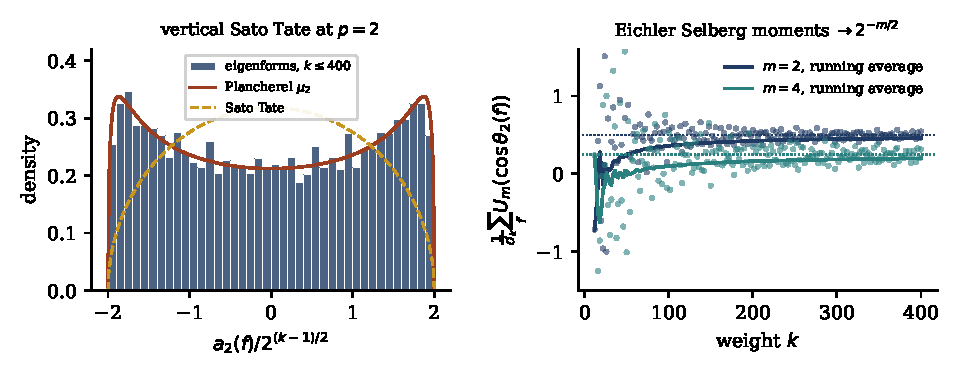
\includegraphics[width=\textwidth]{figs/maass_vertical.pdf}
\caption{Left: Serre's vertical Sato Tate law at $p=2$, the normalised Hecke eigenvalues $a_2(f)/2^{(k-1)/2}$ of the $3234$ level one eigenforms of weight at most $400$ against the Plancherel measure $\mu_2$ of the $3$ regular tree and the Sato Tate law. Right: the empirical moments $\frac1{d_k}\sum_fU_m(\cos\theta_2(f))$ for $m=2$ and $m=4$, computed from the Eichler Selberg formula for every even weight up to $400$ (dots), and their running averages over $k$ (lines), approaching $2^{-m/2}$.}\label{fig:msvertical}
\end{figure}

\section{What this adds to the programme}

The chapter adds the second half of the automorphic spectrum and finds the book's dictionary intact on it: heat trace for explicit formula, eigenvalues for zeros, geodesics for primes, complete monotonicity for the Riemann hypothesis, with Brownian motion on the surface as the probabilistic object that makes the trace formula a statement about return probabilities. It adds two unconditional theorems in the Thorin framework, Theorems~\ref{thm:msthorin} and \ref{thm:mspd}, which are the sine squared lemma and the Poisson Dirichlet theorem for a Beurling system of primes, and one theorem, Theorem~\ref{thm:mscm}, that is the Galois heat trace theorem with the Riemann hypothesis replaced by Selberg's eigenvalue conjecture, and with the complete monotonicity it characterises proved for $\SL_2(\Z)$ and, after the shift of Kim and Sarnak, for every congruence subgroup. It also adds the obstruction of Theorem~\ref{thm:mscm}(iv), which says why the zeros of an $L$ function can be a Thorin measure and the eigenvalues of a surface cannot, and which separates the arithmetic case from the geometric one by a logarithm. Finally it places the even icosahedral problem where it belongs, among the Maass forms of eigenvalue $\frac14$, and shows that the parity of a two dimensional Artin representation is a statement about which gamma factor, holomorphic or Maass, its Galois heat trace wants.

\section{Notes}

Maass introduced his forms in \cite{maass1949} and Selberg the trace formula and the zeta function in \cite{selberg1956}; Hejhal's two volumes \cite{hejhal1976,hejhal1983} and Iwaniec \cite{iwaniec2002} are the references for the noncompact case, and Sarnak's survey \cite{sarnak2003} for the eigenvalue conjecture. McKean's reading of the trace formula through Brownian motion is \cite{mckean1972}; the heat kernel \eqref{eq:msmckean} is there and in Chavel \cite{chavel1984}. The computation of the eigenvalues of $\SL_2(\Z)$ is Hejhal's \cite{hejhal1992}, with rigorous certification by Booker, Str\"ombergsson and Venkatesh \cite{bookerstrombergssonvenkatesh2006}; the values quoted are from the LMFDB \cite{lmfdb}. Weyl's law for $\SL_2(\Z)$ is Selberg's; the lower order terms are in Hejhal. The Kim Sarnak bound is \cite{kimsarnak2003}. The prime geodesic theorem for $\SL_2(\Z)$ and its reading through class numbers is Sarnak \cite{sarnak1982}, reciprocal geodesics are \cite{sarnakreciprocal2007}, and the exponent $\frac{25}{36}$ is Soundararajan and Young \cite{soundararajanyoung2013}. The Eichler Selberg formula is in \cite{eichler1957} and \cite{selberg1956}; the form used is Zagier's, in his appendix to Lang \cite{lang1976} and in \cite{zagier1977}, and the vertical equidistribution is Serre's \cite{serre1997}, with the level one case in Conrey, Duke and Farmer \cite{cdf1997}. Theorems~\ref{thm:mscm}, \ref{thm:msthorin} and \ref{thm:mspd} are new as formulated; their content is Selberg's, Thorin's and Kingman's, assembled through Chapters~\ref{ch:10d}, \ref{ch:recip} and \ref{ch:pd}.

\section{Exercises}

\begin{enumerate}
\item Show that the hyperbolic Brownian motion of Section~\ref{sec:msbm}, started at $i$, has $\E\log y_t=-t$ and that $\log y_t/t\to-1$ almost surely, so that on $\mathbb H$ the process converges to the boundary; explain why on $X$ it does not.
\item Verify from \eqref{eq:msmckean} that $p_t(0)\sim(4\pi t)^{-1}$ as $t\to0$, and that $p_t$ integrates to $1$ over $\mathbb H$.
\item Derive $\pi_\Gamma(x)\sim x/\log x$ from the trace formula with $h(r)=e^{-t(1/4+r^2)}$ as $t\to\infty$, using only $\lambda_0=0$ and $\lambda_1>0$.
\item Show that $R(s)=Z(s+1)/Z(s)$ has a simple pole at $s=1$ with residue $\lim_{s\to1}(s-1)R(s)=Z(2)/Z'(1)$, and compute $Z'(1)$ and $Z(2)$ for the modular surface from the geodesics of norm at most $10^6$.
\item For the Hecke Maass form with $r_1=9.533695$, look up $\lambda(2)$ in the LMFDB, check the Ramanujan bound $|\lambda(2)|\le2$, and write down the Thorin comb of Corollary~\ref{cor:msramanujan}.
\item Prove that the hyperbolic terms of \eqref{eq:msstf} sum to $O(t^{-1/2}e^{-\ell_1^2/4t})$ as $t\to0$, $\ell_1$ the length of the shortest geodesic, so that the identity term alone gives Weyl's law.
\item Using Theorem~\ref{thm:mses}, find all pairs $(k,p)$ with $k\le40$ and $p\le30$ for which $\tr T_p|S_k=0$.
\item Compute $\int U_m(\cos\theta)\,d\mu_p$ for all $m$ and check that the even moments are $p^{-m/2}$.
\end{enumerate}

\section{Open problems}

\begin{problem}[the Thorin representation at the centre]\label{op:mscentre}
Let $R(s)=Z(s+1)/Z(s)$ for a compact surface, and $R^*(s)=(s-1)R(s)$. Determine for which $a\in(0,\frac12)$ the function $R^*(\frac12+a)/R^*(\frac12+a+\sqrt\lambda)$ is, after removal of a drift $e^{|b|\sqrt\lambda}$, the Laplace transform of a GGC, and compute its Thorin density numerically for the Bolza surface or for a Hurwitz surface of small genus, where the spectrum and geodesics are both available. The question is whether the logarithmic divergences of Theorem~\ref{thm:mscm}(iv) cancel into a positive density.
\end{problem}

\begin{problem}[a Chebotarev theorem for geodesics]\label{op:mschebotarev}
Order the primitive geodesics of the modular surface by norm and colour each by the residue of its discriminant $d$ modulo $q$, or by whether $d$ is fundamental. Determine the densities of the colours, prove the Dirichlet process limit of Theorem~\ref{thm:mspd} with that base measure, and identify the analogue of the $L(1,\chi)$ in the Mertens constants. The density of the fundamental discriminants among geodesics ordered by norm is not the density $6/\pi^2$ of fundamental discriminants among all discriminants, because the units weight the count.
\end{problem}

\begin{problem}[even icosahedral representations]\label{op:mseven}
For an even icosahedral Artin representation $\rho$ of conductor $N$ with $\rho(c)=I$ and trivial determinant, so that $\rho$ is self dual, compute the heat trace $\mathcal W^+_\rho$ of Section~\ref{sec:msquarter} from Frobenius traces and test its complete monotonicity numerically, and search for a Maass form of eigenvalue $\frac14$ on $\Gamma_0(N)$ with the Hecke eigenvalues $\tr\rho(\Frob_p)$ by Hejhal's algorithm. A single such form would be the first even icosahedral instance of reciprocity; the computation is within reach for the smallest conductors.
\end{problem}

\begin{problem}[cutoff for Brownian motion on $X(N)$]\label{op:mscutoff}
On the principal congruence covers $X(N)$ the area grows like $N^3$ while $\lambda_1$ stays bounded below by $\frac{975}{4096}$. Determine whether Brownian motion on $X(N)$ started at a fixed point exhibits cutoff in total variation at a time of order $\log N$, as random walks on expander graphs do, and how the cusps, whose number grows with $N$, affect the profile.
\end{problem}

\begin{compproblem}[eigenvalues and geodesics at scale]\label{cp:msspectrum}
Objective: compute the first $10^4$ eigenvalues of $\SL_2(\Z)$ by Hejhal's algorithm with certified error, and the primitive geodesics of norm at most $10^{9}$ from the class numbers and units of the discriminants below $4\cdot10^9$; verify the trace formula for the modular surface, with its elliptic, parabolic and Eisenstein terms, for the heat kernel at $t=0.05$, $0.1$ and $0.2$ to the accuracy of the truncations; and compute the Thorin density of Theorem~\ref{thm:msthorin} at $\alpha=1.1$, where thousands of geodesics contribute. Starting point: \texttt{m1.py} and \texttt{m5.py}.
\end{compproblem}
